\section{Summary}
\label{sec:summary}

\begin{frame}
	\frametitle{To summarise}
	\framesubtitle{XKCD Ineffective Sorts: \url{https://xkcd.com/1185/}}
	\begin{center}
		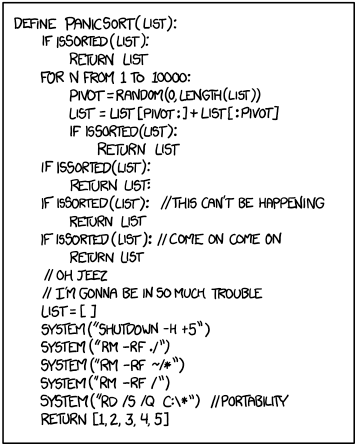
\includegraphics[width=0.4\textwidth]{figures/panicsort.png}\\
	\end{center}
\end{frame}
	
\begin{frame}
	\frametitle{Summary table}
	\begin{tabular}{r | c | c | c}
		\small
		Sorting method & Time & Main advantage & Main disadvantage \\
		\midrule
		Bubble Sort & $O(n^2)$ & Easy for humans! &  Very very very very slow \\
		Insertion Sort & $O(n^2)$ & Good for small lists &  Still quadratic time \\
		Selection Sort & $O(n^2)$ & Good for small lists &  Still quadratic time \\
		Merge Sort & $O(n \log n)$ & Faster than quadratic! &  Bad on `almost sorted lists' \\
		Quick Sort & $O(n \log n)$\footnote{in expectation} & Faster than merge sort &  Still worst-case quadratic\dots \\
	\end{tabular}
	\begin{itemize}
		\item We can mix Bucket Sort in with all this, by applying it first and then applying it (or one of the others) on
			the different buckets.
		\item Sorting algorithms can be in-place or not.
	\end{itemize}
\end{frame}

\begin{frame}
	\frametitle{But wait!}
	\framesubtitle{What about these horses? Where shall I put them?}
	
	\begin{questionblock}{Stable sorting}
		Didn't I also mention stable sorting yesterday?
	\end{questionblock}
	\pause
		\begin{block}{Stable sorting}
			A sorting is stable if: in a list where if $k_i = k_j$ (where $k$ denotes the sorting key,
			e.g. age, or length) and $v_i$ comes for $v_j$ before sorting, then $v_i$ still comes before $v_j$ after sorting.
		\end{block}	
		\pause
			\begin{exampleblock}{Check for yourselves}
				Insertion sort is stable!\\
				Merge sort is not!
			\end{exampleblock}	
\end{frame}

\begin{frame}
	\frametitle{If all else fails}
	\framesubtitle{XKCD Ineffective Sorts: \url{https://xkcd.com/1185/}}
	\begin{quote}
		StackSort connects to StackOverflow, searches for 'sort a list', and downloads and runs code snippets until the list is sorted.
	\end{quote}
	(Mouse-over text for the XKCD linked above).
	\pause
		\begin{exampleblock}{StackSort}
			So of course, someone made this :)\\
			\url{https://gkoberger.github.io/stacksort/}
		\end{exampleblock}	
			\begin{alertblock}{Executing random code!?}
				Use at your own risk (though I did ;))\\
				It does download random bits of code of the Internet and executes them on your computer...
			\end{alertblock}	

	
\end{frame}
